\section{The survey of a sewer - Cloaca Maxima}

\begin{marginfigure}
\begin{tikzpicture}
\node [name-dest] (box){%
    \begin{minipage}{\textwidth}
     \begin{itemize}
    \item Grega Maffi
    \item Tanguy Racine
    \item Clare Tan
    \end{itemize}
    \end{minipage}

};
\node[fancytitle, right=10pt] at (box.north west) {Cloaca Maxima};
\end{tikzpicture}
\end{marginfigure}
The plan was simple: Maffi and I were going to go in Primadona, pick up some rope at Sejna Soba, go in Monatip, then towards the NCB connection and drop a pitch there. Maffi knew the way to the connection given he’d participated in the effort to push the cave during the preceding year. I foolishly assumed he also knew all about Primadona and its connection to Monatip: this is was grave mistake. Still we agreed to meet at the entrance of Primadona the following morning. 
‘What time?’ Maffi asked. Now careful, you must not be seen to offer an easy option, you’re a hard caver.
‘As early as you wish’ I answered. This was not the expected answer, I could see it on Maffi’s face. But then I never really lie in bed.
‘Maybe ten then?’ I offered, as it had become almost a habit to go caving early, in order to come back up for dinner. This time round, dinner in the bivi after the day’s push was not on the cards: it was going to be a long, arduous trip, with glorious, remote exploration involved at some point. Maffi would be coming up from Kal, picking a path through the boulder slope. I would abseil from the top, with the drill, battery and metal work. I couldn’t wait for the trip to begin and the wine did nothing to quench my enthusiasm. Au contraire…

The next morning was quite still, with little wind among the dwarf pine bushes. I found a deserted bivi, all cold grey rock and ash, with pieces of ‘comf’ scattered amongst the remnants of the previous night fire. Even the soothing sound of tarps billowing in the breeze lacked. I rustled up a quick breakfast of biscuits and cheese, cold vitaminski and took it out of the shakehole, to sit on the promontory overlooking M10. 

Then followed the usual shuttle between the tent and the bivi, gathering all the essentials for the coming trip: food, water, gear. Finally it was time to stride across the plateau, to the start of the abseil. 

The silence of the morning was broken by the movement of pebbles underfoot, and soon I clipped into the last drop before the entrance, where Maffi was waiting. I zipped down the rope and we greeted each other, upon which Maffi started to change into his caving gear. As he sat on the grassy ledge, he laid his kit all around him and proceeded to kit up. He had the unfortunate notion of leaning back when putting his socks on: this pushed one of his hiking boots over the edge. I could only look on, clipped to the rope as the shoe rolled down the boulder slope. Even when it was out of sight, the crash of boot on rock could be heard at repeated intervals. 

‘Nooooooo! Why does it have to be me?’ he cried in anguish. 

As far as I knew, the boot might have found its way down to the Tolminka. Still, I offered to climb down to have a look for it, over the first 150 metres of scree that led to the Kuk path. As it happened, the missing item had not gone far and Maffi found it himself, but I had time to climb down to the path and up again before realising that. We spent a surprisingly long time trying to figure out what each other meant: 

‘Tanguy… (non-descript sound) …  up’ 

‘What?’ 

‘… found it …’ 

‘No I haven’t found it! Have you found it?’ 

 ‘… No … up’  
 
‘What?’ 

‘… see it …. up … back’ 

‘Okay I’m going back, Maffi have you found it? I can’t see it’  I couldn’t see the shoe at all, and my wanderings had led me far from the usual access path.

‘No … Come back … I have it’

‘Okay’

I traversed across the scree to get back to the less insane route, climbed up, traversed underneath a little bush of dwarf pine, grabbing the thick, flexible branches as holds, climbed up a little bit more and stopped at a wall of dwarf pine, crowning a small ridge of rock. I hadn’t climbed down this way, but I wasn’t going to let vegetation defeat me. The going got tricky as the slope was steeper than anticipated, and soon I would only be pulling myself up the branches, with little or no footholds. Climbing back down was out of the question, so I had to traverse to the right  hand side, back to the scree slope. I breathed a sigh of relief when I reached the fringe of the pine bush, and carried on up, back to the entrance. 

\begin{figure*}[t!]
\checkoddpage \ifoddpage \forcerectofloat \else \forceversofloat \fi
\centering
\frame{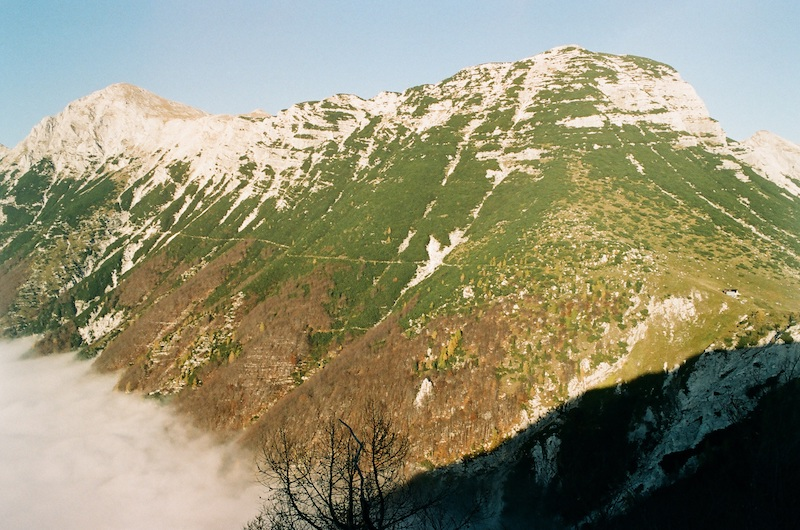
\includegraphics[width=\textwidth]{images/2016/tanguy-sewer-2016/Jarvist_Frost_Mig_from_SW.jpg}}
\caption{Maffi went to Primadona via the 1500m contour path which links Planina na Kalu with Krn on the other side of the valley. Tanguy abseiled down the wester cliffs of the Plateau to meet with him at the cave entrance --- Jarvist Frost}
\label{forest}
\end{figure*}

I was relieved to see that Maffi had found his shoe and after all these tribulations, we were ready to go underground. I pointed out the different branches as we passed them, at Lost and Found junction, at the corkscrew climb, and finally at Sejna Soba. Maffi was quite surprised that, at the time, there were no signs indicating the ways out, or on, or about the cave. Indeed, we’d applied our PSS and paper notes policy to the newly discovered passages and omitted to do the same on the trade routes, relying on our own experience of the cave. This was exactly what had led to memory of the leads, and ways in Primadona to fade in the first place. On a later trip with Tetley, and on his urging a few notes were left at the key junctions insides the cave.

At Sejna Soba Maffi picked up his bag of rope and a small amount of metalwork he’d placed there the previous day on his reconnaissance trip into Primadona. Had I heard that right? It transpired neither of us knew the way to Monatip, other than it was ‘up this rope’ hanging in the main chamber. How difficult could it be though? Monatip was a simple cave, with little in the way of route finding, save at the beginning where the passages leading to NCB had been found.

I ascended first, reaching a very exposed traverse over the chamber into a small rift. There was a carbide arrow leading up to it, and I almost climbed it but Maffi appeared at the pitch head, reading a note in Slovene which said’ traverse more’. The very exposed traverse turned into a madly exposed traverse, leading to yet another small rift, whose only redeeming feature was an exquisite calcified gastropod fossil, weathering out of the rock. The rest was carnage, a tight, sharp draughty rift we had to climb up in, till we broke out into a large aven. There were a few footprints around. The rift continued on the other side of the aven, this led to another chamber, with a possible climb up on the far side. 

The main problem with Monatip was that we expected the way to be hard, mad, dangerous even. This meant we had to try every way up before ascertaining that it really wasn’t ‘the way on’. The climb up was largely vertical, with few footholds and could in no way be attempted without utter disregard for one’s life, so we turned around and explored a few more likely holes, with an entertaining loop I can’t begin to describe. We concluded the way must be somewhere else, so we doubled back down the sinuous tight rift, back to the traverse of death, and traversed more.

As if by magic, the going became easier, and soon we spotted a rope going up an aven. This was it, now we couldn’t get lost! At the top of the pitch, we spotted another rope, and our spirits rose a little. We celebrated victory too quickly though, as the pitch head was a boulder choke, with a possible way down into a boulder strewn  chamber, which we explored. The far side was climbable, but this led through to more wedged boulders that had not seen much passage. With a bit of looking around back the pitch head, I spotted the cairned way on, and we carried on our way up. The boulder choke gave way to a phreatic tube passage, and there was even a Slov PSS by a small round chamber. 

The going was not particularly easy, but we had the draught and the way was well trodden. The passage levelled out and grew bigger, with the signs of an obvious ancient rift streamway going down. Prod marks on the soft mud of the ledges indicated that the way on was up into the rift, and this gained the continuation of the phreatic tube. There, the sediment was churned and flattened by the passage of cavers till we reached a clean-washed aven. With no marks of wellies to indicate the obvious way on, we spent half an hour trying each and hole within this space. We found another oxbow loop, looked everywhere underneath the boulder floor of the aven, but still could not find the way. 

After having a rest, some chocolate and thinking about our predicament, it became evident that we would not complete the through trip from this end of the cave, so we decided to turn back and enter via Monatip to find the way. If we could not push today, at least we would gain valuable knowledge about the cave. 

Somewhat disappointed, we turned around, going down the phreatic tube back to the start of the boulder choke. I started following the cairns but Maffi spotted another neat stack of stones leading away from the pitch head. Curious to see where it led, we soon broke out into a massive aven, which I interpreted to be Alkatraz. This was an opportunity to try out the new route Jack had pioneered early on during the expedition. I found a scramble up boulders on the right hand wall, into a small chamber, and on the opposite side, a little slot through the boulders that was the way down the the Spiral Climb down. 

I reported this back to Maffi, and we opted for the easy way out. Very soon we started motoring up the entrance series of Primadona, and in no time at all, we climbed the snow slope to enjoy the afternoon air on the grassy ledge and gorge on the sight of Krn, the Tolminka valley unfolding beneath us with the faint rush of water far below. We sat there for an hour or so, sharing caving stories and tucking into a nutty fruit mix of Maffi’s own concoction. For a while I tried to guess what was in it - it was after all very fine grained - I got the fig and pistachios after a while but missed the peanut, the linen and sunflower seeds. By all accounts it was delicious, far surpassing the good old raisins and peanuts. 

\begin{figure}[t!]
\checkoddpage \ifoddpage \forcerectofloat \else \forceversofloat \fi
\centering
\frame{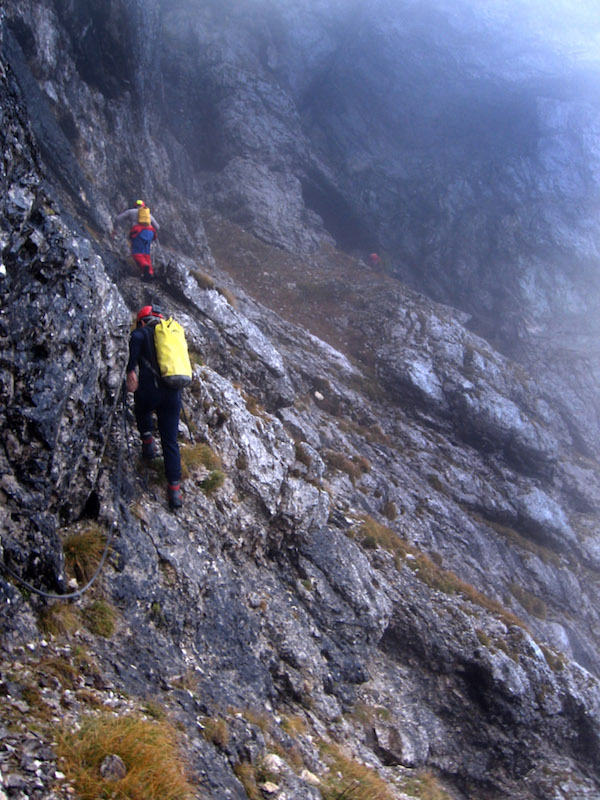
\includegraphics[width=\textwidth]{images/2016/tanguy-sewer-2016/Roped_Entrance_Traverse-Jarv.jpg}}
\caption{The partially protected traverse between Monatip and Primadona is a journey for the faithful --- Jarvist Frost}
\label{traverse}
\end{figure}

We put our gear on again, leaving ropes, metal work and survey kits by the entrance of Monatip in order to travel ‘light’. The cave begins with a pebbly crawl, upwards into the mountain side, branching, before the first pitch. The next section is very straight, with an alternation of abseils, climbs and traverses before reaching the big chamber. Twenty minutes in, we were still only 6 metres below the entrance. The chamber itself is a big aven, with a thin 9mm rope leading up to the connection passages. Maffi led the way up to show me the beginnings of the ‘connection galleries’. The SRT was innovative, with a pitch bypass that allows one to clip in at the highest rebelay, only a few metres before the top. Most of the rocks were loose, and the holds on them were tenuous at best. Still, I was soon shown the start of a long crawl. We turned round there, and descended back to the Big Chamber, where the other way on was the original Monatip rift that had been connected to Primadona at Sejna Soba. 

We scrambled down some huge boulders and entered a small muddy rift. Very early on there is a squeeze which we passed easily, then a window looking into a pitch maybe 20metres deep, then another squeeze best attempted feet first, as it pops out over a drop. At this point, the rift widens, with two broad ledges on either side. Maffi bridged forward a little, and a couple of metres underneath we spotted the ropes going down. Reaching them was going to prove problematic. 

The walls were slick, the good sound holds few and far apart, and we decided that we’d used up all our free climbing enthusiasm for the day. Upon turning around, we spied another passage that merged into the rift, right next to the one we’d come from. Thinking that it could provide us with a safe and sensible way down to the ropes we climbed into it. 
A small upclimb broke through to a small rabbit warren of a chamber, with many phreatic tubes leading off - most being too small to follow. It was a worthy find, but the best was still to come. The obvious way on was the largest phreatic tube, plastered with mud on the floor, with a little film of water on top. We followed the footprints until they stopped. The tube went on.

‘It isn’t obvious anyone’s been here’ I remarked. Further on, the evidence was unequivocal: pristine mud and a thin film of water gathering in little puddles where the erosion had scoured hollows. There was a moderate draught, and although we lacked the survey instruments to survey whatever this passage led to, the thought of discovery spurred us on. 

The tube carried on downwards, at a constant shallow angle, with the same cross-section for a good while until the floor dropped underneath us: this was a small chamber, covered with the same thick, dark mud. From there, a junction of passages: a climb up through smaller tubes which Maffi attempted for a while, the obvious continuation and doubling back under the passage we’d just come from, a muddy crawl which I explored for a couple of metres. 

We opted for the larger, obvious way on, which bent up at a 3m climb, then carried on to reach a T-junction. We chose the downstream end, quickly finding another T-junction, where the passage widened, and opened up. To the right and down, a short section with a deepening rift broke out on the eastern wall of a high, oblong aven. Clean washed boulders on the floor. The sound of drips. 

I whistled in astonishment at our find: the size of the aven was remarkable after such a long time crawling through the tube: near 20x10m cross section at the bottom, and the ceiling lost over 40m higher up. On the western wall, and near the base of the aven, the phreatic conduit beckoned: I had a quick look, and satisfied that it didn’t choke completely after a couple of metres turned around. In the aven, it looked like there could be a twin shaft, connected by a faultplane to the south. This could be accessed by climbing on a boulder pile and bridging the shaft walls where they came close together.

Going out was quick, there was no surveying, no naming without pen, paper and the instruments but from nowhere, we’d found a couple hundred metres of new passage, quite high up in the system. I was thrilled as ever after a discovery and couldn’t wait to go back the next day to survey. There were three guaranteed leads, and many more metres of passage to find, who wouldn’t want to see that?

\name{Tanguy Racine}
